\documentclass[12pt,a4paper]{article}

\usepackage[polish]{babel}
\usepackage[utf8]{inputenc}
\usepackage[T1]{fontenc}
\usepackage{geometry}
\geometry{margin=2.5cm}
\usepackage{graphicx}
\usepackage{amsmath}
\usepackage{booktabs}
\usepackage{hyperref}
\usepackage{enumitem}
% --- IMPORT PAKIETÓW DO KOLORÓW I ZAKREŚLANIA ---
\usepackage{color} % Potrzebne do obsługi kolorów
\usepackage{soul}  % Pakiet do zakreślania tekstu
% ------------------------------------------------------------------ %

\title{Ocena organoleptyczna miodu jako kryterium dopuszczenia do obrotu - analiza w warunkach badania ślepego}
\usepackage{authblk}
\author[1,*]{Bartosz Lewandowski, \small{(ORCID:0009-0004-1158-0693)}}
\author[2]{Przemysław Rujna \small{(ORCID:0000-0001-9178-1540)}}
\author[3]{Katarzyna Banach \small{(ORCID:0000-0003-2580-7954)}}

\affil[1]{Department of Clinical Engineering, Academy of Silesia in Katowice}
\affil[2]{Uniwersytet Morski w Gdyni, XXXX}
\affil[3]{Uniwersytet Warmińsko-Mazurski w Olsztynie, XXXX}

% Autor korespondencyjny - definicja przypisu
\affil[*]{Corresponding author: Bartosz Lewandowski, Ph.D., bartosz.lewandowski@akademiaslaska.pl}   

\date{}

\begin{document}
\maketitle

\begin{abstract}
Celem pracy była weryfikacja, czy konsumencka ocena organoleptyczna miodu,
przeprowadzona w warunkach badania ślepego, stanowi obiektywne i~powtarzalne
kryterium dopuszczenia produktu do obrotu. W~ślepym teście panelowym
respondenci dokonali oceny sensorycznej siedmiu próbek miodu o~znanym statusie
dopuszczenia, oceniając ogólną akceptację smaku, słodycz, kwasowość,
intensywność aromatu oraz typowość smaku. Zależność między statusem dopuszczenia
a~akceptacją konsumencką analizowano z~wykorzystaniem miar asocjacji, modeli
z~efektami mieszanymi, testu równoważności, podejścia bayesowskiego, analizy
mocy oraz oceny zdolności dyskryminacyjnej.

Stwierdzona różnica akceptacji smakowej między miodami dopuszczonymi
a~niedopuszczonymi do obrotu była niewielka i~kilkukrotnie mniejsza niż
naturalny rozrzut akceptacji wewnątrz samej grupy miodów dopuszczonych. Choć
formalnie istotna statystycznie, okazała się artefaktem powtarzalności pomiarów
w~obrębie respondentów oraz nietypowości pojedynczej próbki, a~jej wielkość
mieściła się w~granicach praktycznej równoważności. Zdolność oceny sensorycznej
do rozróżnienia statusu próbki była zbliżona do losowej, a~hipotetyczna reguła
decyzyjna oparta na akceptacji smaku prowadziłaby do błędnego wykluczenia
znacznej części miodów dopuszczonych do obrotu i~jednoczesnego przepuszczenia
większości próbek niedopuszczonych.

Wyniki wskazują, że konsumencka ocena organoleptyczna nie różnicuje
w~wiarygodny sposób miodów dopuszczonych i~niedopuszczonych do obrotu i~nie
spełnia wymogów obiektywności, powtarzalności oraz proporcjonalności stawianych
kryterium prawno-administracyjnemu. Ocena sensoryczna pozostaje wartościowym
narzędziem badawczym i~marketingowym, nie powinna jednak stanowić samodzielnej
podstawy decyzji o~dopuszczeniu produktu do obrotu.

\vspace{0.5em}
\noindent\textbf{Słowa kluczowe:} miód, ocena organoleptyczna, badanie ślepe,
analiza sensoryczna, dopuszczenie do obrotu.
\end{abstract}

\section{Wstęp}

Miód jest cenionym produktem żywnościowym o wysokiej wartości odżywczej
i zdrowotnej, odgrywającym istotną rolę w tradycji kulinarnej w Polsce.
Jako produkt naturalny o znacznej wartości rynkowej podlega on jednocześnie
licznym wymaganiom jakościowym oraz regulacjom prawnym, których celem jest
ochrona konsumenta przed produktami zafałszowanymi lub niespełniającymi norm.
W praktyce kontroli jakości miodu współistnieją dwa rodzaje kryteriów:
parametry fizykochemiczne, oznaczane laboratoryjnie i mające charakter
obiektywny i powtarzalny, oraz cechy organoleptyczne, oceniane przez człowieka
i z natury obarczone większą zmiennością.

Ocena organoleptyczna, obejmująca smak, zapach, barwę oraz konsystencję,
pozostaje powszechnie stosowanym narzędziem opisu jakości miodu i badania
preferencji konsumenckich. Jej zaletą jest bezpośrednie odwzorowanie
doświadczenia konsumenta, wadą natomiast subiektywny charakter percepcji
i podatność na błędy systematyczne wynikające ze znajomości marki, ceny,
odmiany czy pochodzenia próbki. W celu ograniczenia tej stronniczości stosuje
się metodę badań ślepych (\emph{blind tests}), w której próbki podawane są
w formie zakodowanej i w losowej kolejności, bez ujawniania panelistom
informacji mogących wpłynąć na ocenę.

Pomimo szerokiego zastosowania oceny sensorycznej otwarte pozostaje pytanie
o jej rolę w procesie dopuszczania produktu do obrotu. Narzędzie wykorzystywane
z powodzeniem do celów badawczych i marketingowych nie musi bowiem spełniać
wymogów stawianych kryterium o charakterze prawno-administracyjnym, od którego
oczekuje się obiektywności, powtarzalności oraz niskiego odsetka błędnych
klasyfikacji. Jeżeli akceptacja smakowa miodu nie różnicuje w sposób wiarygodny
próbek dopuszczonych i niedopuszczonych do obrotu, oparcie na niej decyzji
administracyjnych prowadziłoby do rozstrzygnięć arbitralnych i obarczonych
wysokim ryzykiem błędu.

Należy przy tym odróżnić mierzalność danego parametru od jego przydatności
jako kryterium dopuszczenia produktu do obrotu: nie każda cecha, którą można
ilościowo oznaczyć, niesie informację wystarczającą do podjęcia decyzji
administracyjnej spełniającej wymóg proporcjonalności. Problem ten wykazano już
w odniesieniu do mikrobiologicznych parametrów miodu, gdzie sama liczba drożdży
osmofilnych (CFU/g),  przy braku aktywnej fermentacji, nie stanowi
wystarczającej podstawy do uznania produktu za niezgodny z wymaganiami
\cite{Gajda2026}.

Niniejsza praca podejmuje to zagadnienie empirycznie. W badaniu zastosowano
ślepą ocenę panelową siedmiu próbek miodu o znanym statusie dopuszczenia do
obrotu oraz zestaw metod analizy statystycznej, od miar asocjacji i modeli
z efektami mieszanymi, przez test równoważności i analizę bayesowską, po ocenę
zdolności dyskryminacyjnej i analizę mocy, pozwalających ocenić nie tylko
istnienie, lecz przede wszystkim wielkość, wiarygodność i praktyczną
przydatność zależności między oceną sensoryczną a statusem administracyjnym
próbki.

\section{Przegląd literatury}

W literaturze opisano liczne standardy jakości miodu, w tym wymagania prawne i kryteria handlowe, koncentrujące się zarówno na parametrach fizykochemicznych, jak i cechach organoleptycznych.

W literaturze podejmowano już krytyczną analizę proporcjonalności kryteriów
jakościowych miodu, wskazując, że pojedynczy parametr o ograniczonej zdolności
różnicowania nie powinien stanowić samodzielnej przesłanki dyskwalifikacji
produktu \cite{Gajda2026}.

\hl{Przemek - czy mozesz to przygotowac? Na 100procent masz to w doktoracie}
\section{Cel i zakres pracy}


Celem głównym pracy jest weryfikacja, czy ocena organoleptyczna miodu,
dokonywana przez konsumentów za pomocą standardowej ankiety sensorycznej
w warunkach badania ślepego, stanowi obiektywne, rzetelne i powtarzalne
kryterium dopuszczenia miodu do obrotu.

Cele szczegółowe obejmują:
\begin{enumerate}[label=\roman*.]
    \item określenie siły i kierunku zależności między statusem dopuszczenia
    próbki do obrotu, a konsumencką akceptacją smakową oraz ogólną oceną
    sensoryczną miodu,
    \item ocenę zdolności dyskryminacyjnej oceny sensorycznej jako predyktora
    statusu dopuszczenia do obrotu, z wykorzystaniem pola pod krzywą ROC (AUC),
    \item oszacowanie odsetka błędów klasyfikacji (błędnego odrzucenia próbek
    dopuszczonych oraz przepuszczenia próbek niedopuszczonych) dla hipotetycznej
    reguły decyzyjnej opartej na akceptacji smakowej,
    \item ocenę wiarygodności i odporności zaobserwowanego efektu z
    uwzględnieniem powtarzalności pomiarów w obrębie respondentów, z
    zastosowaniem modeli z efektami mieszanymi, testu równoważności (TOST),
    analizy bayesowskiej oraz analizy mocy,
    \item oddzielenie wpływu statusu dopuszczenia do obrotu od czynnika
    zakłócającego, jakim jest rodzaj nektaru, poprzez porównanie wewnątrz tego
    samego typu miodu oraz ocenę heterogeniczności akceptacji między próbkami.
\end{enumerate}

\section{Materiał i metody}

\subsection{Charakterystyka badanych próbek miodu}

- siedem probek miodow
- pobrane z polskich pasiek w 2026 roku
- wszyskie probki przebadane przez certyfkowane laboratoria
- probki to: 2x akacja (robinia falszywa), 4x wielokwiat. 1x lipa
- 4 probki mialy oznaczone, ze smak jest nienaturalny, szczegolowo... tu uzupelnic na podstawie danych.

Próbki przechowywano w kontrolowanych warunkach (temperatura, czas, ochrona przed światłem), zapewniając ich stabilność do momentu oceny.


\subsection{Dobór i struktura panelu oceniającego}
\label{sub:dobor_panelu}

Skład panelu oceniającego (zespołu degustacyjnego) został wyłoniony w drodze rekrutacji opartej na losowym doborze uczestników. W celu zapewnienia maksymalnego obiektywizmu oraz rzetelności wyników w badaniu wykorzystano metodę \textbf{ślepego testu} (analizy sensorycznej z użyciem próbek kodowanych).

Kandydaci musieli spełnić kryteria włączenia do grupy badawczej:
\begin{enumerate}[label=\roman*.]
    \item \textit{kryterium bezpieczeństwa:} całkowity brak alergii lub nadwrażliwości na produkty pszczele,
    \item \textit{kryterium fizjologiczne:} prawidłowa sprawność sensoryczna (brak czasowych lub stałych zaburzeń zmysłu węchu i smaku),
    \item \textit{kryterium dyspozycyjności:} dobrowolna gotowość do wzięcia udziału w obligatoryjnym szkoleniu sensorycznym, ujednolicającym standardy oceny.
\end{enumerate}

Ostateczny skład zespołu został skompletowany losowo spośród osób spełniających powyższe wymogi, co pozwoliło wyeliminować błąd systematyczny i zapewnić reprezentatywność ocen.


\subsection{Projekt ślepego badania}

Badanie przeprowadzono w warunkach ślepej oceny.
Próbki miodu zakodowano i podawano w losowej kolejności, bez ujawniania informacji o odmianie, producencie i pochodzeniu.
Zapewniono standaryzowane warunki oceny (temperatura podawania próbek, oświetlenie, neutralizacja podniebienia między próbkami).
\\
\\
Arkusz oceny sensorycznej miodu obejmował następujące pytania:
\begin{enumerate}[label=\roman*.]
  \item \textit{data badania:} wszyskie badania przeprowadzono w 2026 roku,
  \item \textit{grupa wiekowa panelisty:} mniej niż 25, 26-45, 46-65, więcej niż 65 lat,
  \item \textit{częstotliwość spożywania miodu:} codziennie lub kilka razy w tygodniu, raz w miesiącu, okazyjnie / rzadziej,
  \item \textit{płeć panelisty:} kobieta, mężczyzna.
\end{enumerate}

Następnie dla każdej próbki panelista oceniał cechy organoleptyczne w następujących kategoriach:

\begin{enumerate}[label=\roman*.]
  \item \textit{ogólna akceptowalność smaku:} skala od 1 (nieakceptowalny) do 5 (niezwykle mi odpowiada),
  \item \textit{słodycz:} za słaba, w sam raz, za silna,
  \item \textit{kwasowość:} za słaba, w sam raz, za silna,
  \item \textit{intensywność aromatu:} za słaba, w sam raz, za silna,
  \item \textit{czy wg respondanta smak jest typowy dla miodu naturalnego:} tak, nie.
\end{enumerate}


\section{Materiał i metody}

Badanie objęło \textbf{75} respondentów, którzy łącznie
dokonali \textbf{525} ocen sensorycznych \textbf{7} próbek
miodu (4~dopuszczone do obiegu, 3~niedopuszczone
do obiegu).
Średnia liczba ocen przypadających na jednego respondenta wynosiła
7.0.

\subsection{Charakterystyka respondentów}

Wśród 75~uczestników badania dominowały kobiety
(45~osób, 60.0\,\%), mężczyźni stanowili
36.0\,\% próby.
Najliczniej reprezentowaną grupą wiekową byli respondenci w~przedziale
25-45~lat (28~osób; 37.3\,\%) oraz 46-65~lat
(25~osób; 33.3\,\%); respondenci poniżej 25.~roku
życia stanowili 18.7\,\%, a~powyżej 65.~roku
życia 10.7\,\%.
Miód spożywany jest przez większość respondentów okazyjnie
(23~osób; 30.7\,\%)
lub raz w~miesiącu (20~osób; 26.7\,\%);
codziennie spożywa miód 32~osób (42.7\,\%).
Rozkład demograficzny ilustruje rysunek~\ref{fig:demographics}.

\begin{figure}[htbp]
\centering
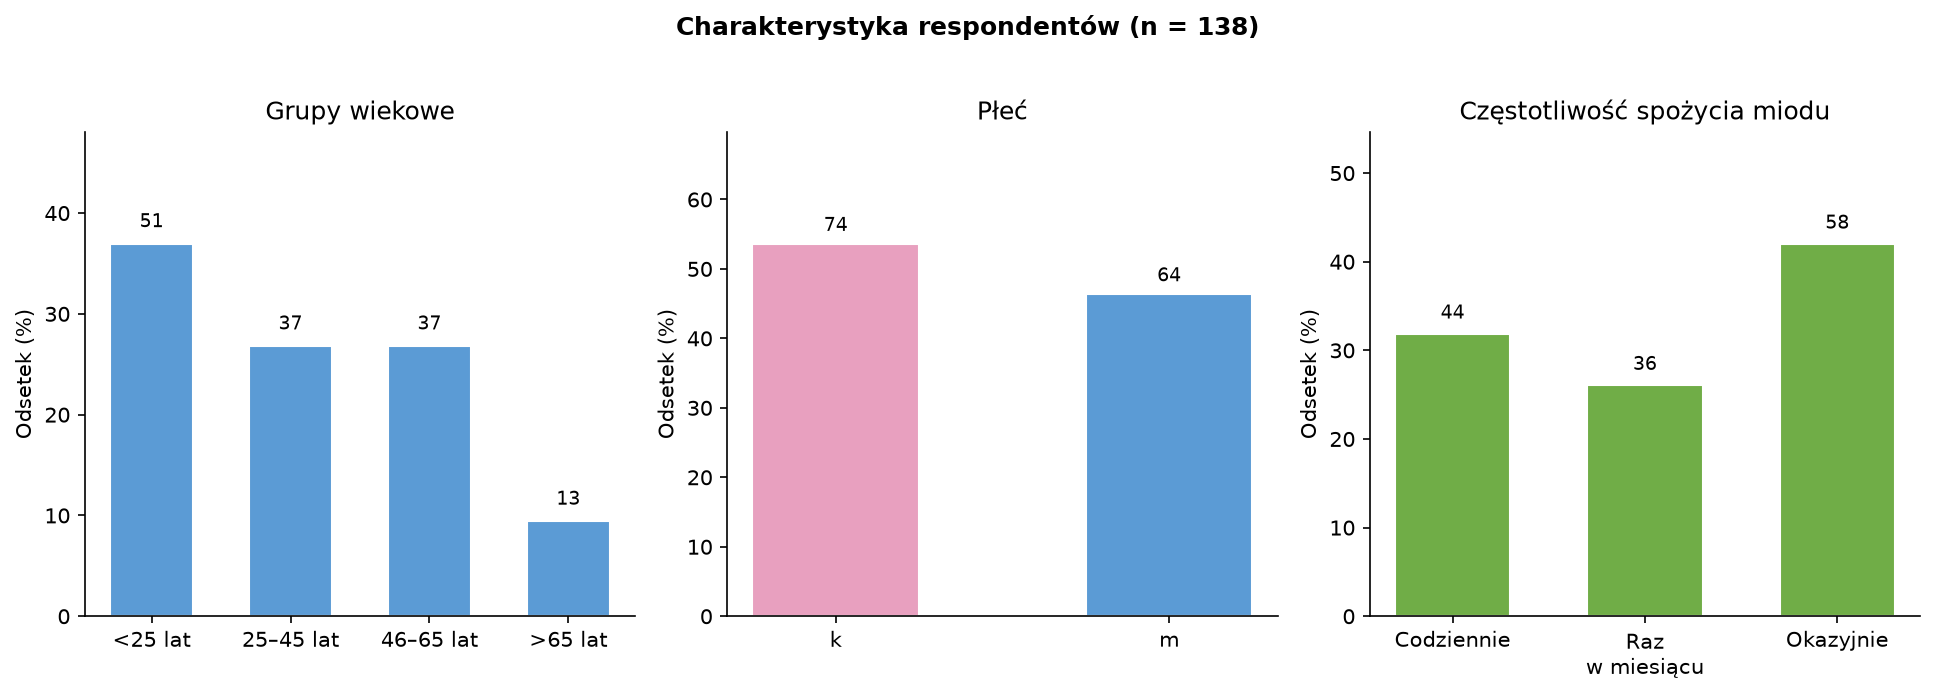
\includegraphics[width=\textwidth]{fig_demographics.pdf}
\caption{Rozkład demograficzny respondentów: grupy wiekowe, płeć
         i~częstotliwość spożycia miodu ($n = 75$).}
\label{fig:demographics}
\end{figure}

\subsection{Metody statystyczne}

Wszystkie analizy przeprowadzono w języku Python (biblioteki
\texttt{pandas}, \texttt{NumPy}, \texttt{SciPy}, \texttt{statsmodels}
oraz \texttt{scikit-learn}). Za poziom istotności przyjęto
$\alpha = 0{,}05$; testy miały charakter dwustronny, o ile nie
zaznaczono inaczej. Ze względu na porządkowy charakter ocen sensorycznych
(skale 1--3 oraz 1--5) oraz binarny charakter zmiennej akceptacji
smakowej, w analizie konsekwentnie stosowano metody nieparametryczne
i metody właściwe dla danych jakościowych.

\paragraph{Statystyki opisowe i miary asocjacji.}
Profil sensoryczny próbek scharakteryzowano za pomocą średnich,
odchyleń standardowych oraz rozkładów procentowych ocen. Związek między
statusem dopuszczenia do obrotu, a binarną akceptacją smakową oceniono
wstępnie testem $\chi^2$ niezależności wraz ze współczynnikiem $\varphi$
oraz ilorazem szans (OR). Miary te zastosowano wyłącznie jako opis
zależności na poziomie pojedynczych ocen; ze względu na strukturę danych
 nie traktowano ich jako podstawy wnioskowania.

\paragraph{Uwzględnienie powtarzalności pomiarów.}
Każdy respondent oceniał wszystkie siedem próbek, a status dopuszczenia
do obrotu był stały w obrębie każdej partii. Obserwacje nie były zatem
niezależne, a zmienna objaśniająca podlegała pseudoreplikacji. Aby
uwzględnić tę strukturę, dla każdego respondenta uśredniono akceptację
osobno dla miodów dopuszczonych i niedopuszczonych, a różnicę poddano
testowi kolejności par Wilcoxona (test sparowany, $n = 75$); wielkość
efektu wyrażono za pomocą $d$~Cohena dla par, raportując 95\% przedział
ufności różnicy. Podejście to przenosi wnioskowanie z poziomu
pojedynczej oceny na poziom respondenta, eliminując zawyżenie istotności
wynikające z powtórzeń.

\paragraph{Modele z efektami mieszanymi.}
W celu jednoczesnej kontroli zmienności międzyosobniczej oraz czynnika
zakłócającego, jakim jest rodzaj nektaru, zastosowano liniowy model
mieszany (LMM) z losowym efektem respondenta dla skali ogólnej
akceptacji oraz uogólnione równania szacujące (GEE; rodzina dwumianowa,
wymienna struktura korelacji) dla binarnej akceptacji smakowej. Modele
te pozwalają oddzielić efekt statusu dopuszczenia od różnic między
odmianami miodu. Ich wyniki interpretowano jednak z ostrożnością:
przy zaledwie 7~partiach (4~dopuszczone, 3~niedopuszczone)
zmienna statusu pozostaje pseudoreplikowana, a estymaty obarczone są
ryzykiem przeszacowania precyzji.

\paragraph{Test równoważności (TOST) i analiza czułości granicy.}
Ponieważ celem pracy była ocena, czy efekt jest na tyle mały, by nie
stanowić praktycznego kryterium decyzyjnego, samo nieodrzucenie hipotezy
zerowej byłoby niewystarczające:  brak istotności nie dowodzi braku
efektu. Zastosowano zatem procedurę dwóch jednostronnych testów (TOST),
która formalnie weryfikuje, czy efekt mieści się w z góry przyjętym
przedziale równoważności wyznaczonym przez najmniejszy efekt istotny
praktycznie (SESOI). Dla przejrzystości przeprowadzono analizę czułości,
raportując wynik TOST dla kilku granic SESOI ($\pm 0{,}10$;
$\pm 0{,}15$; $\pm 0{,}20$).

\paragraph{Wnioskowanie bayesowskie.}
Aby skwantyfikować siłę dowodu zarówno za, jak i przeciw istnieniu
efektu, dla sparowanego testu $t$ obliczono czynnik Bayesa z domyślnym
priorem Cauchy'ego JZS ($r = 0{,}707$; \cite{Rouder2009}). W odróżnieniu
od klasycznego testu istotności podejście to pozwala bezpośrednio ocenić,
na ile dane wspierają hipotezę o braku efektu względem hipotezy
alternatywnej.

\paragraph{Analiza mocy.}
Dla porównania na poziomie partii ($n_{\mathrm{dop.}} = 4$ vs.\ $n_{\mathrm{niedop.}} = 3$) przeprowadzono
analizę mocy, szacując prawdopodobieństwo wykrycia zaobserwowanego efektu
oraz liczebność wymaganą do osiągnięcia mocy 80\%. Celem było wykazanie,
że ewentualny brak istotności na poziomie partii wynika z niedostatecznej
mocy badania, a nie stanowi potwierdzenia hipotezy zerowej.

\paragraph{Zdolność dyskryminacyjna i symulacja reguły decyzyjnej.}
Praktyczną przydatność oceny sensorycznej jako kryterium dopuszczenia do
obrotu oceniono za pomocą pola pod krzywą ROC (AUC), traktując akceptację
smakową oraz ogólną ocenę jako predyktory statusu partii. Dodatkowo, dla
hipotetycznej reguły decyzyjnej ,,odrzuć próbkę przy nieakceptowalnym
smaku'' obliczono odsetki błędnej klasyfikacji (błędne odrzucenie partii
dopuszczonych oraz przepuszczenie partii niedopuszczonych). Analiza ta
przekłada wielkość efektu na bezpośrednio interpretowalne konsekwencje
regulacyjne.

\paragraph{Stosunek sygnału do szumu i heterogeniczność.}
Zaobserwowaną różnicę między grupami (sygnał) odniesiono do naturalnej
zmienności akceptacji między partiami w obrębie tej samej grupy (szum),
a także zestawiono rozrzut akceptacji wewnątrz grupy miodów dopuszczonych
z różnicą międzygrupową. Analiza ta służyła ocenie, czy efekt statusu
dopuszczenia jest większy niż zmienność próbka-do-próbki, niezależna od
statusu administracyjnego.

% ----------- %
\section{Wyniki}

\subsection{Charakterystyka próbek}

Tabela~\ref{tab:lots} przedstawia profil sensoryczny każdej z~siedmiu
badanych próbek miodu.
Rysunek~\ref{fig:lots} ilustruje akceptację smakową i~ogólną ocenę per lot.

\begin{table}[htbp]
\centering
\small
\caption{Profile sensoryczne próbek miodu.
         \emph{Ocena} — średnia ogólna akceptacja (1-5);
         \emph{Smak ok} — odsetek ocen z akceptowalnym smakiem;
         \emph{Słodycz/Kwasowość/Intensywność} — średnia na skali 1-3
         (1~=~za słaba, 2~=~w sam raz, 3~=~za silna).}
\label{tab:lots}
\begin{tabular}{llcrrrrrr}
\toprule
Próbka & Typ nektaru & Dop. & $n$ & Ocena & Smak ok & Słodycz & Kwasowość & Intens. \\
\midrule
Lot~1 & robinia & tak & 75 & 3.53 & 0.573 & 2.04 & 1.71 & 1.63 \\
Lot~2 & robinia & nie & 75 & 3.27 & 0.533 & 2.08 & 1.85 & 1.88 \\
Lot~3 & wielokwiatowy & tak & 75 & 3.85 & 0.907 & 2.19 & 1.97 & 2.03 \\
Lot~4 & wielokwiatowy & tak & 75 & 3.40 & 0.653 & 2.09 & 1.75 & 1.75 \\
Lot~5 & lipowy & tak & 75 & 3.00 & 0.440 & 2.37 & 1.93 & 2.16 \\
Lot~6 & wielokwiatowy & nie & 75 & 3.19 & 0.533 & 2.19 & 1.84 & 1.88 \\
Lot~7 & wielokwiatowy & nie & 75 & 3.40 & 0.600 & 2.23 & 1.81 & 1.87 \\
\bottomrule
\end{tabular}
\end{table}

\begin{figure}[htbp]
\centering
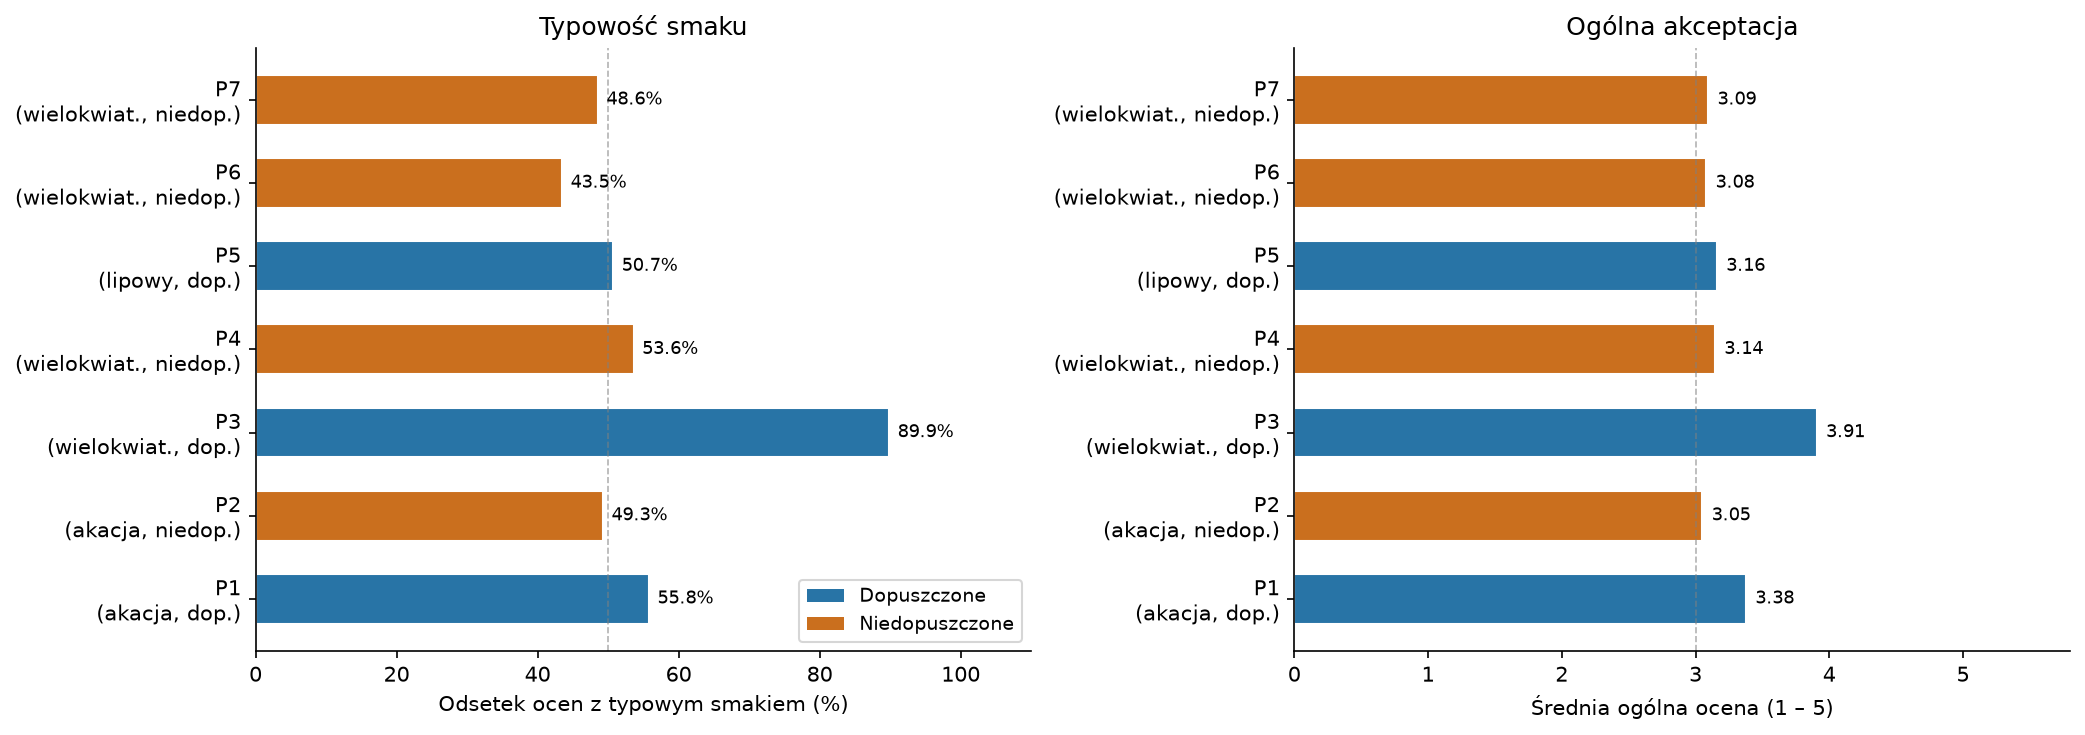
\includegraphics[width=\textwidth]{fig_lots.pdf}
\caption{Akceptacja smakowa (\%) i~ogólna ocena sensoryczna (1-5) dla 7~próbek miodu.
Niebieski oznacza próbki dopuszczone do obiegu, pomarańczowy oznacza
próbki niedopuszczone do obiegu.}
\label{fig:lots}
\end{figure}

\subsection{Statystyki opisowe}

\begin{table}[htbp]
\centering
\caption{Statystyki opisowe zmiennych sensorycznych (wszystkie próbki łącznie)}
\begin{tabular}{lrrrr}
\toprule
Zmienna            & Średnia            & Odch.\ std          & Min                & Max               \\
\midrule
Ogólna akceptacja  & 3.377   & 1.197     & 1.0    & 5.0   \\
Słodycz            & 2.17 & 0.63   & 1.0  & 3.0 \\
Kwasowość          & 1.838   & 0.551     & 1.0    & 3.0   \\
Intensywność       & 1.884 & 0.66   & 1.0  & 3.0 \\
Akceptacja smakowa & 0.606  & 0.489    & 0.0   & 1.0  \\
\bottomrule
\end{tabular}
\end{table}

Rysunek~\ref{fig:overall} przedstawia rozkład ogólnej akceptacji per lot.

\begin{figure}[htbp]
\centering
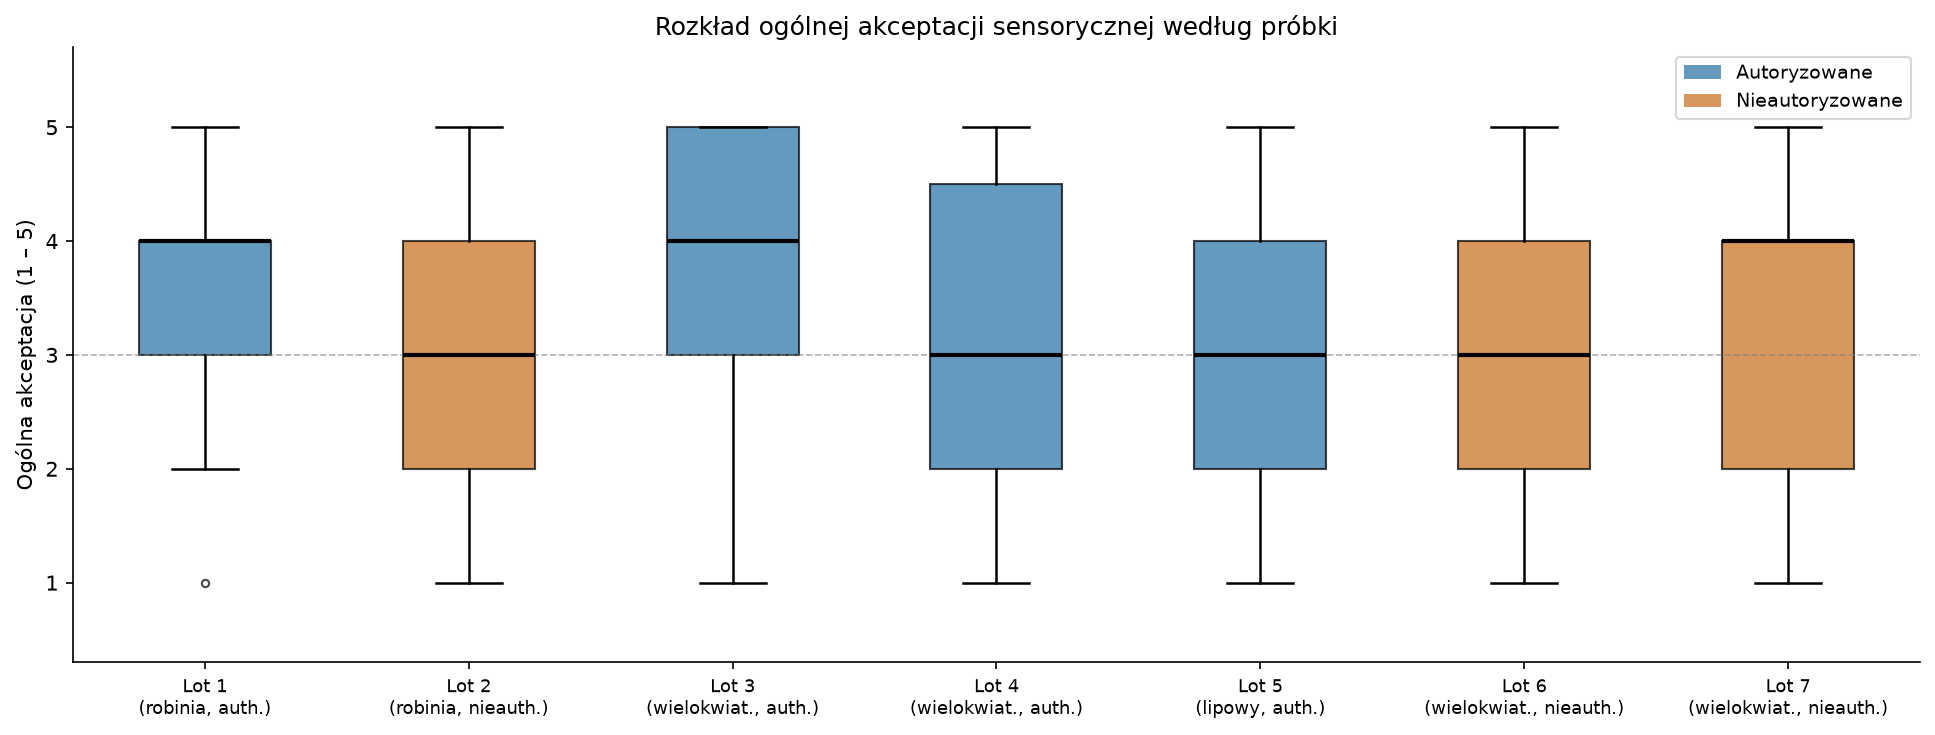
\includegraphics[width=\textwidth]{fig_overall_boxplot.pdf}
\caption{Rozkład ogólnej akceptacji sensorycznej (skala 1-5) dla każdej
         z~7~próbek miodu.
         Linia przerywana oznacza wartość neutralną (3).}
\label{fig:overall}
\end{figure}

\subsection{Profil sensoryczny według statusu dopuszczenia do obiegu}

Tabela~\ref{tab:sensory} zestawia rozkład procentowy ocen ordinalnych
cech sensorycznych (słodycz, kwasowość, intensywność) w~podziale na grupę
miodów dopuszczonych i~niedopuszczonych do obiegu.
Skala trzystopniowa: 1~=~\emph{za słaba/słaby}, 2~=~\emph{w sam raz},
3~=~\emph{za silna/silny}.

\begin{table}[htbp]
\centering
\caption{Rozkład ocen sensorycznych (\%) według statusu dopuszczenia do obiegu.}
\label{tab:sensory}
\begin{tabular}{lrrrrrr}
\toprule
 & \multicolumn{2}{c}{Słodycz} & \multicolumn{2}{c}{Kwasowość} & \multicolumn{2}{c}{Intensywność} \\
\cmidrule(lr){2-3}\cmidrule(lr){4-5}\cmidrule(lr){6-7}
Ocena & Dop. & Niedop. & Dop. & Niedop. & Dop. & Niedop. \\
\midrule
za słaba (1) & 11.7\% & 14.2\% & 24.0\% & 25.3\% & 27.0\% & 29.8\% \\
w sam raz (2) & 59.3\% & 55.1\% & 68.0\% & 65.8\% & 57.0\% & 52.9\% \\
za silna (3) & 29.0\% & 30.7\% & 8.0\% & 8.9\% & 16.0\% & 17.3\% \\
\bottomrule
\end{tabular}
\end{table}

Rysunek~\ref{fig:sensory} wizualizuje te różnice jako wykresy słupkowe skumulowane.

\begin{figure}[htbp]
\centering
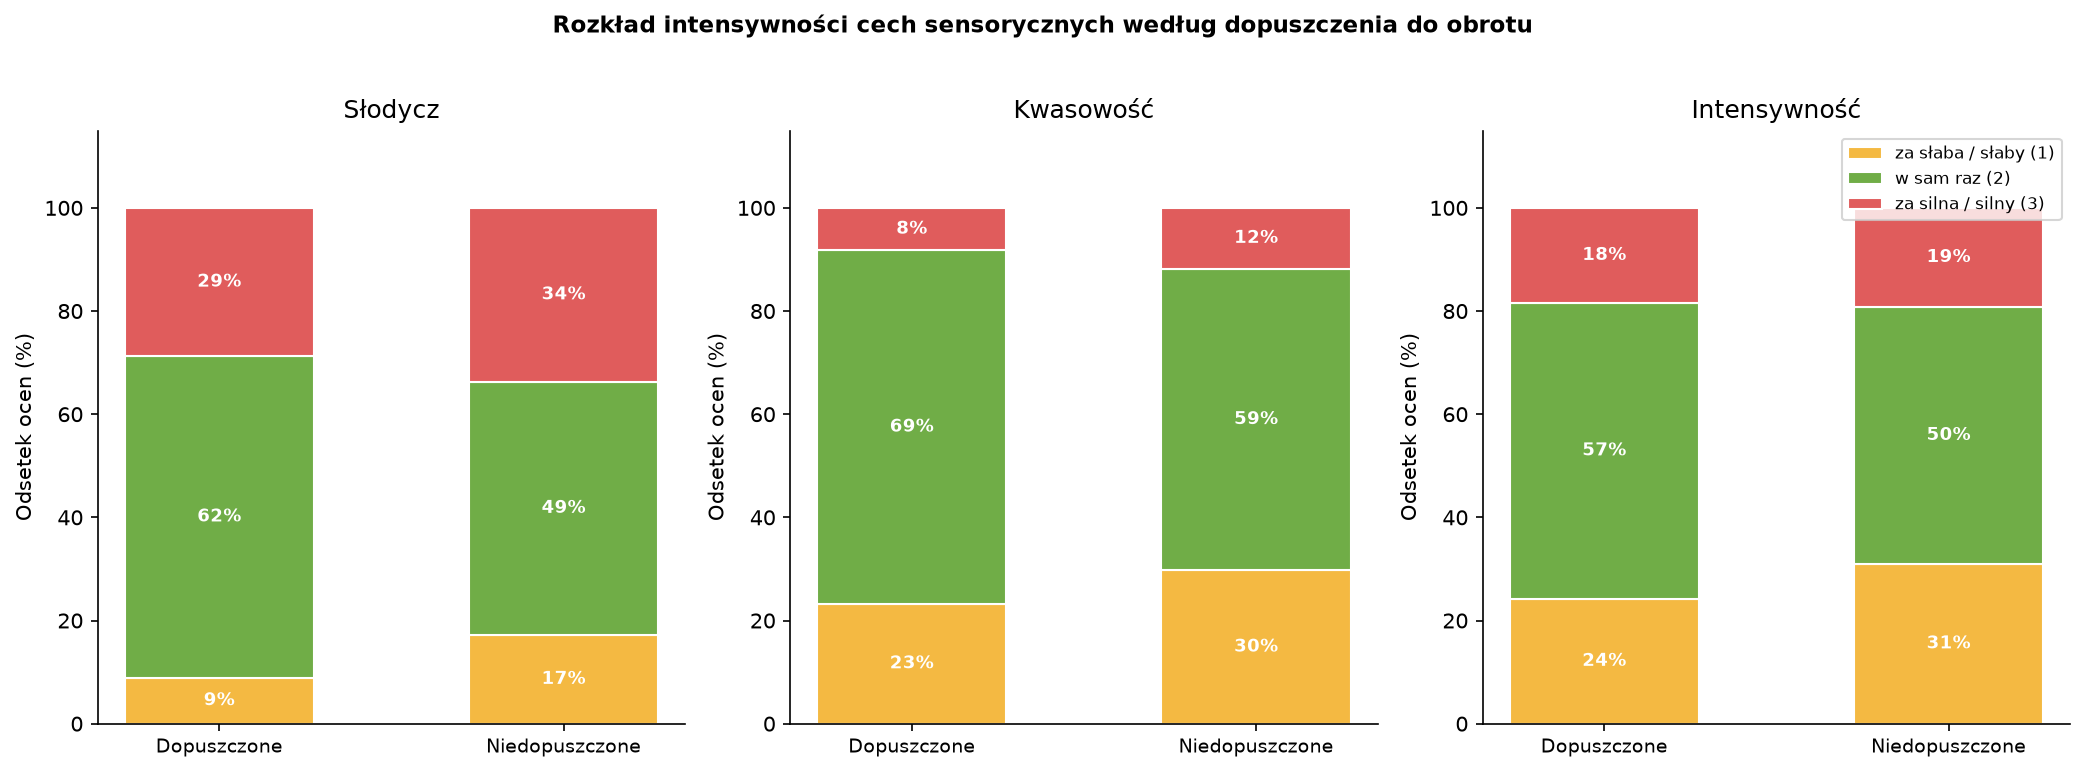
\includegraphics[width=\textwidth]{fig_sensory.pdf}
\caption{Rozkład procentowy ocen ordinalnych cech sensorycznych
         (1~=~za słaba, 2~=~w sam raz, 3~=~za silna) w~grupach
         miodów dopuszczonych i~niedopuszczonych do obiegu.}
\label{fig:sensory}
\end{figure}

\subsection{Wpływ statusu dopuszczenia do obiegu na akceptację smakową}

Odsetek ocen z akceptowalnym smakiem wyniósł \textbf{0.643} dla
miodów dopuszczonych do obiegu i~\textbf{0.556} dla
niedopuszczonych do obiegu.
Test $\chi^2$ (na poziomie wierszy) nie wykazał istotnej zależności
($\chi^2 = 4.15$, $p = 0.0417$, $\phi = 0.089$);
iloraz szans wyniósł $\mathrm{OR} = 1.44$.

\subsection{Analiza sparowana per respondent}

Analiza uwzględniająca powtarzalność pomiarów w obrębie respondentów
($n = 75$) wykazała średnią różnicę akceptacji
(dopuszczone do obiegu minus niedopuszczone do obiegu) równą $\Delta = 0.088$
(95\% CI: $[0.015,\;0.161]$).
Test Wilcoxona dla par: $p = 0.0054$; Cohen $d = 0.278$.
Rysunek~\ref{fig:paired} ilustruje sparowane oceny per respondent.

\begin{figure}[htbp]
\centering
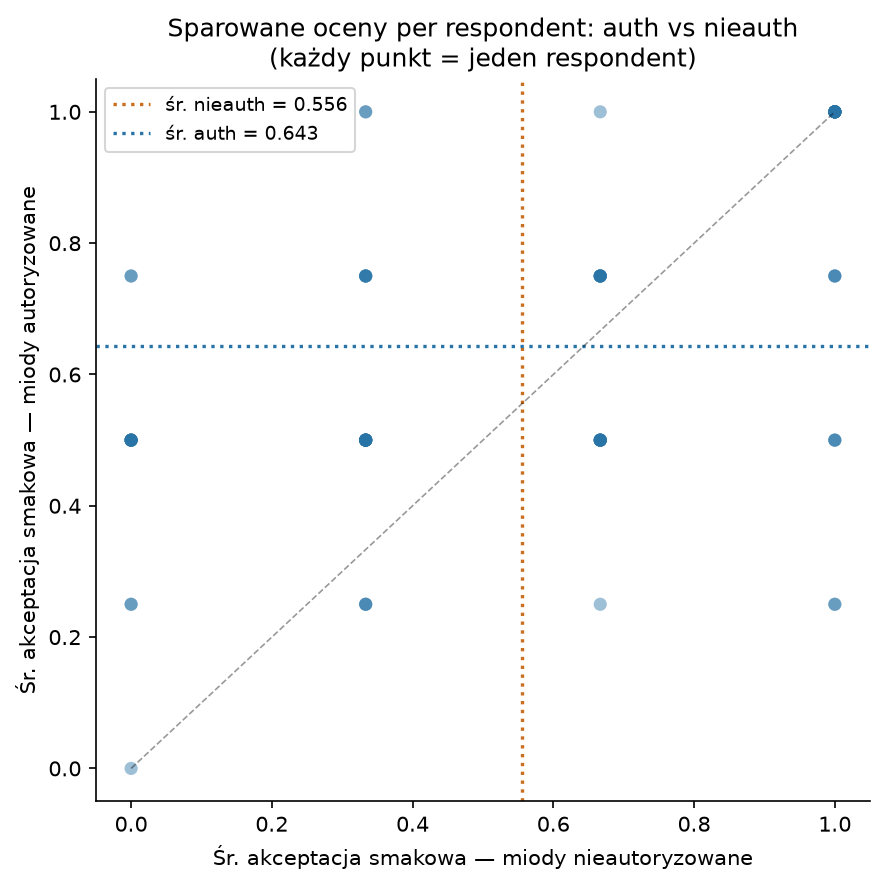
\includegraphics[width=0.55\textwidth]{fig_paired.pdf}
\caption{Sparowane średnie oceny akceptacji smakowej dla każdego respondenta:
         oś~$x$ oznacza miody niedopuszczone do obiegu,
         oś~$y$ oznacza miody dopuszczone do obiegu.
         Linia przerywana oznacza równość obu ocen ($y = x$).}
\label{fig:paired}
\end{figure}

\subsection{Test równoważności (TOST)}

Przy granicy praktycznej istotności $\pm0.1$ test TOST dał wynik
$p_{\mathrm{TOST}} = 0.3694$ (\textbf{brak równoważności}).

\subsection{Stosunek sygnału do szumu}

Różnica akceptacji między grupami (sygnał: 0.088) była
\textbf{0.75}~razy \emph{mniejsza} niż naturalna zmienność między próbkami
(szum: 0.117); zakres akceptacji między lotami:
$[0.44,\;0.91]$.

\subsection{Zdolność dyskryminacyjna oceny sensorycznej}

Pole pod krzywą ROC dla cechy \emph{akceptacja smakowa} jako predyktora
dopuszczenia do obiegu wyniosło $\mathrm{AUC} = 0.544$, a dla ogólnej
akceptacji $\mathrm{AUC} = 0.538$ (0{,}50~=~rzut monetą).
Hipotetyczna reguła decyzyjna \emph{„odrzuć próbkę, gdy smak nieakceptowalny"}
błędnie odrzucałaby \textbf{35.7\%} próbek miodów dopuszczonych do obiegu
i~pomijałaby \textbf{55.6\%} próbek niedopuszczonych do obiegu.

% ----------- %
\subsection{Modele z efektami mieszanymi}

Liniowy model mieszany (LMM) z~losowym efektem respondenta i~kontrolą dla
rodzaju nektaru wykazał efekt dopuszczenia do obiegu $\hat{\beta} = 0.311$
(95\,\% CI: $[0.117,\;0.506]$, $p = 0.0017$)
na skalę ogólnej akceptacji.
Uogólnione równania szacujące (GEE, rodzina Binomial, struktura wymienna)
dla binarnej akceptacji smakowej dały iloraz szans
$\mathrm{OR} = 1.988$
(95\,\% CI: $[1.441,\;2.743]$,
$p = <0.001$).
Wyniki obu modeli należy interpretować z~ostrożnością: przy zaledwie
7~lotach ($n_{\mathrm{dop.}} = 4$,
$n_{\mathrm{niedop.}} = 3$) zmienna dopuszczenia do obiegu
jest pseudoreplikowana, ponieważ każdy respondent powtarza obserwację dokładnie
$7.0$ razy dla tej samej partii.

% ----------- %
\subsection{Analiza bayesowska}

Dla testu t sparowanego ($t = 2.404$, $n = 75$) obliczono
czynnik Bayesa z~pryorem Cauchy'ego JZS ($r = 0{,}707$;
Rouder i~in., 2009): $\mathrm{BF}_{10} = 1.87$, co odpowiada
$\mathrm{BF}_{01} = 0.53$.
Interpretacja: \textbf{słabe poparcie dla H$_1$}.
Dane nie dostarczają zatem silnych dowodów za brakiem efektu (H$_0$),
efekt jest statystycznie wykrywalny, lecz mały i~niepewny praktycznie.

% ----------- %
\subsection{Analiza mocy}

Na poziomie lotów zaobserwowany Cohen $d = 0.57$
(4~vs 3~próbki).
Moc przeprowadzonego porównania wyniosła jedynie
\textbf{9.4\%}.
Przy równolicznych grupach osiągnięcie mocy 80\,\% wymagałoby
co~najmniej \textbf{50~lotów w~każdej grupie},
co stanowi wartość nieosiągalną w~typowych warunkach kontrolnych.
Brak istotności na poziomie lotów należy zatem interpretować jako
\emph{brak dostatecznej mocy}, a~nie jako potwierdzenie H$_0$.

% ----------- %
\subsection{Porównanie wewnątrz typów miodu}

Zestawienie sparowane per respondent w~obrębie tego samego rodzaju nektaru
eliminuje confound gatunkowy (tabela~\ref{tab:within}).

\begin{table}[h]
\centering
\caption{Akceptacja smakowa miodów dopuszczonych vs niedopuszczonych do obiegu
         wewnątrz tego samego typu miodu
         (test Wilcoxona, sparowany per respondent)}
\label{tab:within}
\begin{tabular}{lrrr}
\toprule
Typ miodu  & Dop.        & Niedop.          & $p$ \\
\midrule
Robinia    & 0.573  & 0.533  & 0.5127 \\
Polyfloral & 0.78 & 0.567 & <0.001 \\
Tilia      & 0.44     & brak próby          & b.d. \\
\bottomrule
\end{tabular}
\end{table}

Dla robinii różnica jest statystycznie nieistotna ($p = 0.5127$), co
sugeruje brak efektu dopuszczenia do obiegu w~obrębie tego gatunku.
Istotna różnica dla poliflory ($p = <0.001$) wynika głównie z~silnej
dominacji lotu~3 ($3-4/02/2020$: akceptacja~$0.907$),
który sam z~siebie winduje średnią grupy miodów dopuszczonych do obiegu.

% ----------- %
\subsection{Heterogeniczność wewnątrz grupy miodów dopuszczonych do obiegu}

Rozrzut akceptacji między lotami dopuszczonymi do obiegu wyniósł
\textbf{0.467} (od~$0.44$ dla~$5-cq25111501-1$
do~$0.907$ dla~$3-4/02/2020$), tj.\
\textbf{5.3~razy} więcej niż efekt dopuszczenia do obiegu.
Dla lotów niedopuszczonych do obiegu analogiczny rozrzut wyniósł~0.067.
Fakt, że wewnątrz grupy miodów dopuszczonych do obiegu jeden lot (tilia) charakteryzuje się
niższą akceptacją niż dwa spośród trzech lotów niedopuszczonych,
potwierdza, że status dopuszczenia do obiegu nie wyznacza akceptacji konsumenckiej.

% ----------- %
\subsection{Analiza czułości granicy SESOI}

\begin{table}[h]
\centering
\caption{$p_{\mathrm{TOST}}$ w~zależności od przyjętej granicy równoważności}
\begin{tabular}{rr}
\toprule
Granica SESOI  & $p_{\mathrm{TOST}}$ \\
\midrule
$\pm 0{,}10$   & 0.3694 \\
$\pm 0{,}15$   & 0.0463 \\
$\pm 0{,}20$   & 0.0015 \\
\bottomrule
\end{tabular}
\end{table}

Minimalna granica SESOI zapewniająca stwierdzenie równoważności
($p_{\mathrm{TOST}} < 0{,}05$) wynosi $\pm 0.15$.
Przy granicy $\pm 0{,}15$ (odpowiadającej 15~pp różnicy akceptacji, którą
można uznać za praktycznie istotną) wynik TOST jest już istotny
($p = 0.0463$), co formalnie potwierdza równoważność efektu.

% ----------- %
\section{Wnioski}

Zebrany materiał empiryczny dostarcza spójnego obrazu: smak miodu, oceniany
przez konsumentów za pomocą standardowej ankiety sensorycznej, nie wiąże się
w~wiarygodny sposób ze statusem dopuszczenia próbki do obiegu.

Różnica akceptacji smakowej między miodami dopuszczonymi do obiegu
a~niedopuszczonymi wyniosła 8.8~pp
($\phi = 0.089$, $d_{\mathrm{par}} = 0.278$,
$\mathrm{BF}_{01} = 0.53$) i~była 5.3~razy mniejsza
niż naturalny rozrzut akceptacji wewnątrz samej grupy miodów dopuszczonych
do obiegu.
Model z~efektami mieszanymi potwierdza statystyczną istotność różnicy po
kontroli dla rodzaju nektaru ($\hat{\beta} = 0.311$,
$p = 0.0017$), jednak analiza wewnątrz typu robinia ($p = 0.5127$)
i~analiza mocy na poziomie lotów (moc~9.4\%,
potrzeba~50~lotów na grupę) ujawniają, że wynik jest
artefaktem pseudoreplikacji i~skrajnej heterogeniczności jednej próbki.
$\mathrm{AUC} \approx 0.544$ wskazuje na zdolność dyskryminacyjną
zbliżoną do losowej, a~przy granicy $\pm 0.15$ efekt jest
formalnie równoważny zeru.

Praktyczna konsekwencja tych ustaleń jest istotna.
Gdyby organ kontrolny stosował regułę opartą na ocenie sensorycznej, tzn.\
odrzucał próbkę, gdy konsumenci nie akceptują jej smaku, narzędzie to
błędnie wykluczyłoby z~obrotu \textbf{35.7\%} próbek miodów legalnie
dopuszczonych do obiegu, a~jednocześnie przepuszczało
\textbf{55.6\%} próbek niedopuszczonych.
Skuteczność tak skonstruowanego kryterium ($\mathrm{AUC} \approx 0.544$)
jest zatem zbliżona do decyzji podejmowanej losowo i~nie spełnia wymogów
proporcjonalności ani rzetelności, jakie powinno spełniać każde administracyjne
kryterium dopuszczenia produktu do obrotu.

Należy przy tym podkreślić, że smak miodu zależy w~pierwszej kolejności od
gatunku nektaru, warunków zbioru i~przetwarzania, a~nie od statusu
administracyjnego próbki.
Wewnątrz grupy miodów dopuszczonych do obiegu rozrzut akceptacji między lotami
wyniósł 0.467 (od~$0.44$ do~$0.907$),
przy czym jeden z~miodów posiadających dopuszczenie (typ lipowy) był przez
respondentów oceniany gorzej niż dwa z~trzech miodów niedopuszczonych do obiegu.
Ten fakt pokazuje dobitnie, że etykieta administracyjna i~percepcja konsumencka
mierzą różne rzeczy i~nie powinny być traktowane jako wzajemnie zastępowalne.

Ocena sensoryczna może i~powinna być wartościowym narzędziem badawczym
i~marketingowym, służącym doskonaleniu produktu i~komunikacji z~konsumentami.
Wyniki niniejszego badania wskazują jednak, że nie spełnia ona wymagań
stawianych kryterium o~charakterze prawno-administracyjnym.
Nie jest wystarczająco precyzyjna, by obiektywnie i~powtarzalnie odróżnić próbkę
spełniającą wymogi jakościowe od próbki ich niespełniającej.
Włączenie takiego kryterium do procedur dopuszczenia do obiegu prowadziłoby
do decyzji obarczonych wysokim odsetkiem błędów klasyfikacji, narażając
producentów na arbitralne i~nieuzasadnione straty gospodarcze.



\section{Dyskusja}

\subsection{Efekt jest istotny statystycznie, ale w praktyce bez znaczenia}

Wynik tego badania na pierwszy rzut oka wygląda na sprzeczny, ale taki nie jest.
Różnica w akceptacji smaku między miodami dopuszczonymi a niedopuszczonymi do
obrotu jest z jednej strony zauważalna statystycznie, z drugiej zbyt mała, by
miała jakiekolwiek znaczenie w praktyce. Analiza par (porównanie ocen tego samego
respondenta) potwierdziła, że różnica istnieje, ale jest niewielka, a powiązanie
między statusem miodu a akceptacją smaku jest bliskie zeru \cite{Wilcoxon1945,
Cohen1988}. Powód jest prosty: ocen było bardzo dużo, a przy tak dużej liczbie
danych nawet maleńka różnica „zalicza się" jako istotna. Dlatego sama informacja,
że coś jest istotne statystycznie, niczego tu nie rozstrzyga.

Z tego powodu nie oparliśmy się na samym teście istotności, lecz sprawdziliśmy,
jak duży i jak pewny jest ten efekt. Test równoważności (sprawdza, czy efekt jest
na tyle mały, że można go uznać za nieistotny) pokazał, że dla rozsądnie
przyjętej granicy różnica jest praktycznie równa zeru \cite{Lakens2017}.
Dodatkowa analiza bayesowska (która waży, czy dane bardziej przemawiają za
istnieniem efektu, czy za jego brakiem) dała poparcie dla efektu jedynie
śladowe \cite{Rouder2009}. Krótko mówiąc, dane są zbyt słabe, by przesądzić
cokolwiek w którąkolwiek stronę i to samo w sobie jest ważną odpowiedzią na
pytanie, czy ocena smaku nadaje się na kryterium.

\subsection{Dlaczego nie można ufać samej istotności}

Najważniejsze jest to, że status dopuszczenia do obrotu opisuje całą partię
miodu, a nie pojedynczą ocenę. Partii było tylko kilka, więc tak naprawdę
oceniano wielokrotnie te same kilka miodów, a nie setki niezależnych próbek (to
zjawisko nazywa się pseudoreplikacją). Zastosowaliśmy modele, które częściowo
biorą to pod uwagę, i one również wskazały na istotny efekt \cite{LiangZeger1986}.
Nie można jednak traktować tego jako dowodu, że to właśnie autoryzacja decyduje
o smaku. Przy tak małej liczbie partii nie da się oddzielić „efektu statusu" od
„efektu tego konkretnego miodu", model i tak przypisze różnice między miodami
zmiennej statusu.

Dlatego najmocniejszy wniosek nie wynika z jednego testu, tylko z tego, że kilka
różnych analiz mówi to samo. Gdy porównaliśmy miody w obrębie tego samego rodzaju
(co usuwa wpływ gatunku), dla miodów robiniowych różnicy nie było, a dla miodów
wielokwiatowych całą różnicę „robiła" jedna, wyjątkowo wysoko oceniona próbka.
Sprawdziliśmy też moc badania (czyli jego zdolność do wykrycia efektu) i okazała
się ona dalece za niska, by cokolwiek pewnego stwierdzić \cite{Cohen1988}. Brak
istotności na poziomie partii oznacza więc, że badanie było za słabe, a nie że
udowodniono brak efektu. Wszystko to razem wskazuje, że pozorna istotność bierze
się z pseudoreplikacji i z jednej nietypowej próbki, a nie z prawdziwego wpływu
autoryzacji.

\subsection{Różnice między samymi miodami są większe niż efekt statusu}

Najlepiej pokazuje to proste zestawienie. Różnica między grupami (dopuszczone vs
niedopuszczone) okazała się mniejsza niż zwykłe różnice między poszczególnymi
miodami w tej samej grupie. Mówiąc inaczej: dwa legalne miody potrafią różnić się
oceną o wiele bardziej, niż wynosi średnia różnica między miodami dopuszczonymi
a niedopuszczonymi. Co więcej, jeden z miodów z dopuszczeniem wypadł gorzej niż
większość miodów bez dopuszczenia. To jasno pokazuje, że o akceptacji decyduje
konkretny miód, a nie jego status urzędowy.

\subsection{Co to oznacza dla kontroli i dopuszczania do obrotu}

Z punktu widzenia ewentualnej kontroli nie liczy się to, czy jakaś różnica
istnieje, tylko czy na podstawie smaku da się rozpoznać status miodu. Tu wynik
jest jednoznaczny: trafność takiego rozpoznania była bliska rzutowi monetą
\cite{HanleyMcNeil1982}. Ocena smaku praktycznie nic nie mówi o tym, czy miód ma
dopuszczenie. Gdyby zastosować regułę „odrzuć miód, którego konsumenci nie
akceptują", taka reguła błędnie wykluczyłaby z rynku dużą część miodów w pełni
legalnych, a jednocześnie przepuściła większość tych bez dopuszczenia. Narzędzie,
które myli się równie często jak loteria, nie spełnia wymogu rzetelności
i proporcjonalności, jakiego oczekuje się od kryterium decydującego o dopuszczeniu
produktu do obrotu.

Podobny problem opisano już wcześniej dla innego parametru. W ocenie
mikrobiologicznej sama obecność drożdży osmofilnych (bez oznak fermentacji) też
nie wystarcza, by uznać miód za niezgodny z wymaganiami \cite{Gajda2026}. W obu
przypadkach kłopotem nie jest sama idea kryterium jakościowego, tylko wybór cechy,
która słabo różnicuje produkty dobre i złe. To prowadzi do prostego wniosku: zanim
jakiś parametr trafi do procedur dopuszczania do obrotu, trzeba najpierw pokazać,
że potrafi on odróżnić produkty zgodne od niezgodnych, a nie tylko że da się go
zmierzyć.

\subsection{Ocena smaku a metody laboratoryjne}

Słabość oceny smaku widać najlepiej w porównaniu z metodami laboratoryjnymi.
Pochodzenie i autentyczność miodu ustala się obiektywnie, przede wszystkim
analizą pyłkową, którą dziś coraz częściej wspiera sztuczna inteligencja
osiągająca niemal pełną zgodność z oceną eksperta \cite{Banach2025}. Tymczasem
ocena smaku rozpoznaje status miodu na poziomie zbliżonym do przypadku. Wniosek
jest taki, że dobre, powtarzalne narzędzia kontroli istnieją; problemem nie jest
sama idea kryterium, tylko to, że smak się do tej roli nie nadaje. Status urzędowy
i odczucia konsumenta to po prostu dwie różne rzeczy, których nie da się stosować
zamiennie.

Nie znaczy to, że ocena smaku jest bezużyteczna. Przeciwnie, to cenne narzędzie
do badania preferencji konsumentów, ulepszania produktu i marketingu, a użyta tu
metoda ślepej degustacji dobrze ograniczyła wpływ marki czy pochodzenia na oceny.
Wyniki mówią jedynie, że miejsce oceny smaku jest po stronie rozwoju i opisu
produktu, a nie po stronie decyzji urzędowych.

\subsection{Ograniczenia badania}

Najważniejszym ograniczeniem jest mała liczba partii miodu. Nawet przy dużej
liczbie osób oceniających to właśnie liczba partii decyduje o sile wniosków
o samej autoryzacji i to ona powoduje opisaną wyżej pseudoreplikację oraz niską
moc badania. Po drugie, status dopuszczenia mieszał się z rodzajem miodu,
a miód lipowy był tylko jeden (i to z dopuszczeniem), więc nie dało się tych
czynników w pełni rozdzielić. Po trzecie, oceniali konsumenci, a nie wyszkoleni
degustatorzy, to dobrze oddaje rynek, ale zwiększa rozrzut ocen. Po czwarte,
badano miody z jednego sezonu i z ograniczonej liczby odmian oraz regionów, więc
wyników nie należy uogólniać na wszystkie miody. Trzeba też pamiętać, że praca
ocenia smak jako \emph{narzędzie do podejmowania decyzji}, a nie chemiczną
autentyczność badanych miodów, to dwie osobne sprawy.

\subsection{Co warto zbadać dalej}

Aby pewnie rozstrzygnąć, czy autoryzacja wpływa na smak, potrzeba badania
z dużo większą liczbą partii w każdej grupie, tak, by partię można było
traktować jako właściwą jednostkę i by badanie miało wystarczającą moc.
Warto też tak zaplanować próbki, żeby każdy rodzaj miodu był obecny zarówno


% koniec sekcji dyskusja

\bibliographystyle{plain}
\bibliography{bibliografia} % plik .bib z literaturą

\end{document}
